
\subsection{Our voltage regulation circuit}

Our purpose was to regulate voltages and also study noise related to the circuit. If we choose a complicated circuit for voltage voltage regulation then analysis of noise will be relatively complicated. So, we used a very basic voltage regulator circuit from a zener diode. Supply was given as DC power supply with voltage $V_{s}$. This voltage is decided by the zener voltage at hand.

The noise in the circuit will be relatively higher at the zener breakdown region. As we discussed from the theoretical part, noise power will be proportional to current flowing in the zener diode (here, we are assuming that noise from other parts is almost zero). To prepare a zener diode (BZX55C5V1) to break down the region we choose 5.4V. This is calculated from 
For our purpose we utilised a general purpose zener diode with breakdown region between 4.8V to 5.4V with current of $\mu A$ order. We first did the Current and voltage characteristics of zener diodes. The useful information we got from there is source voltages, zener voltages and current that we particularly needed in our project. Our aim was to never exceed the LOCK IN amplifier’s input limits. Current and voltage characteristics are down in figure \ref{exiv}. The zener diode we used had its datasheets, which you can see from Appendix. Its power rating is … 

\begin{figure}[hbt!]
\centering{\centering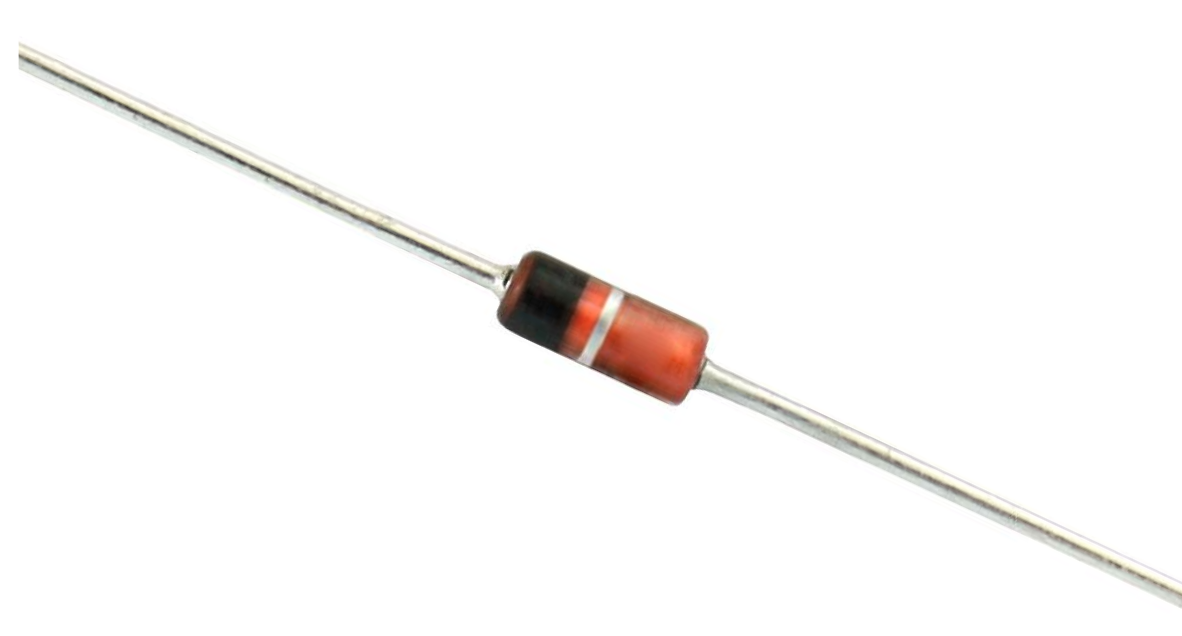
\includegraphics[width=.48\textwidth]{zener.png}}
\caption{Our zener diode}
\end{figure}

The zener diode was given proper voltages to work in reverse bias, specifically in the breakdown region. The overall circuit was identical to that of voltage regulator by zener diode. We gave particularly 5.0 V, 5.5V in two different runs from the powersource. The Zener diode regulated around 4.9 V. 

\begin{figure*}[hbt!]
\centering{\centering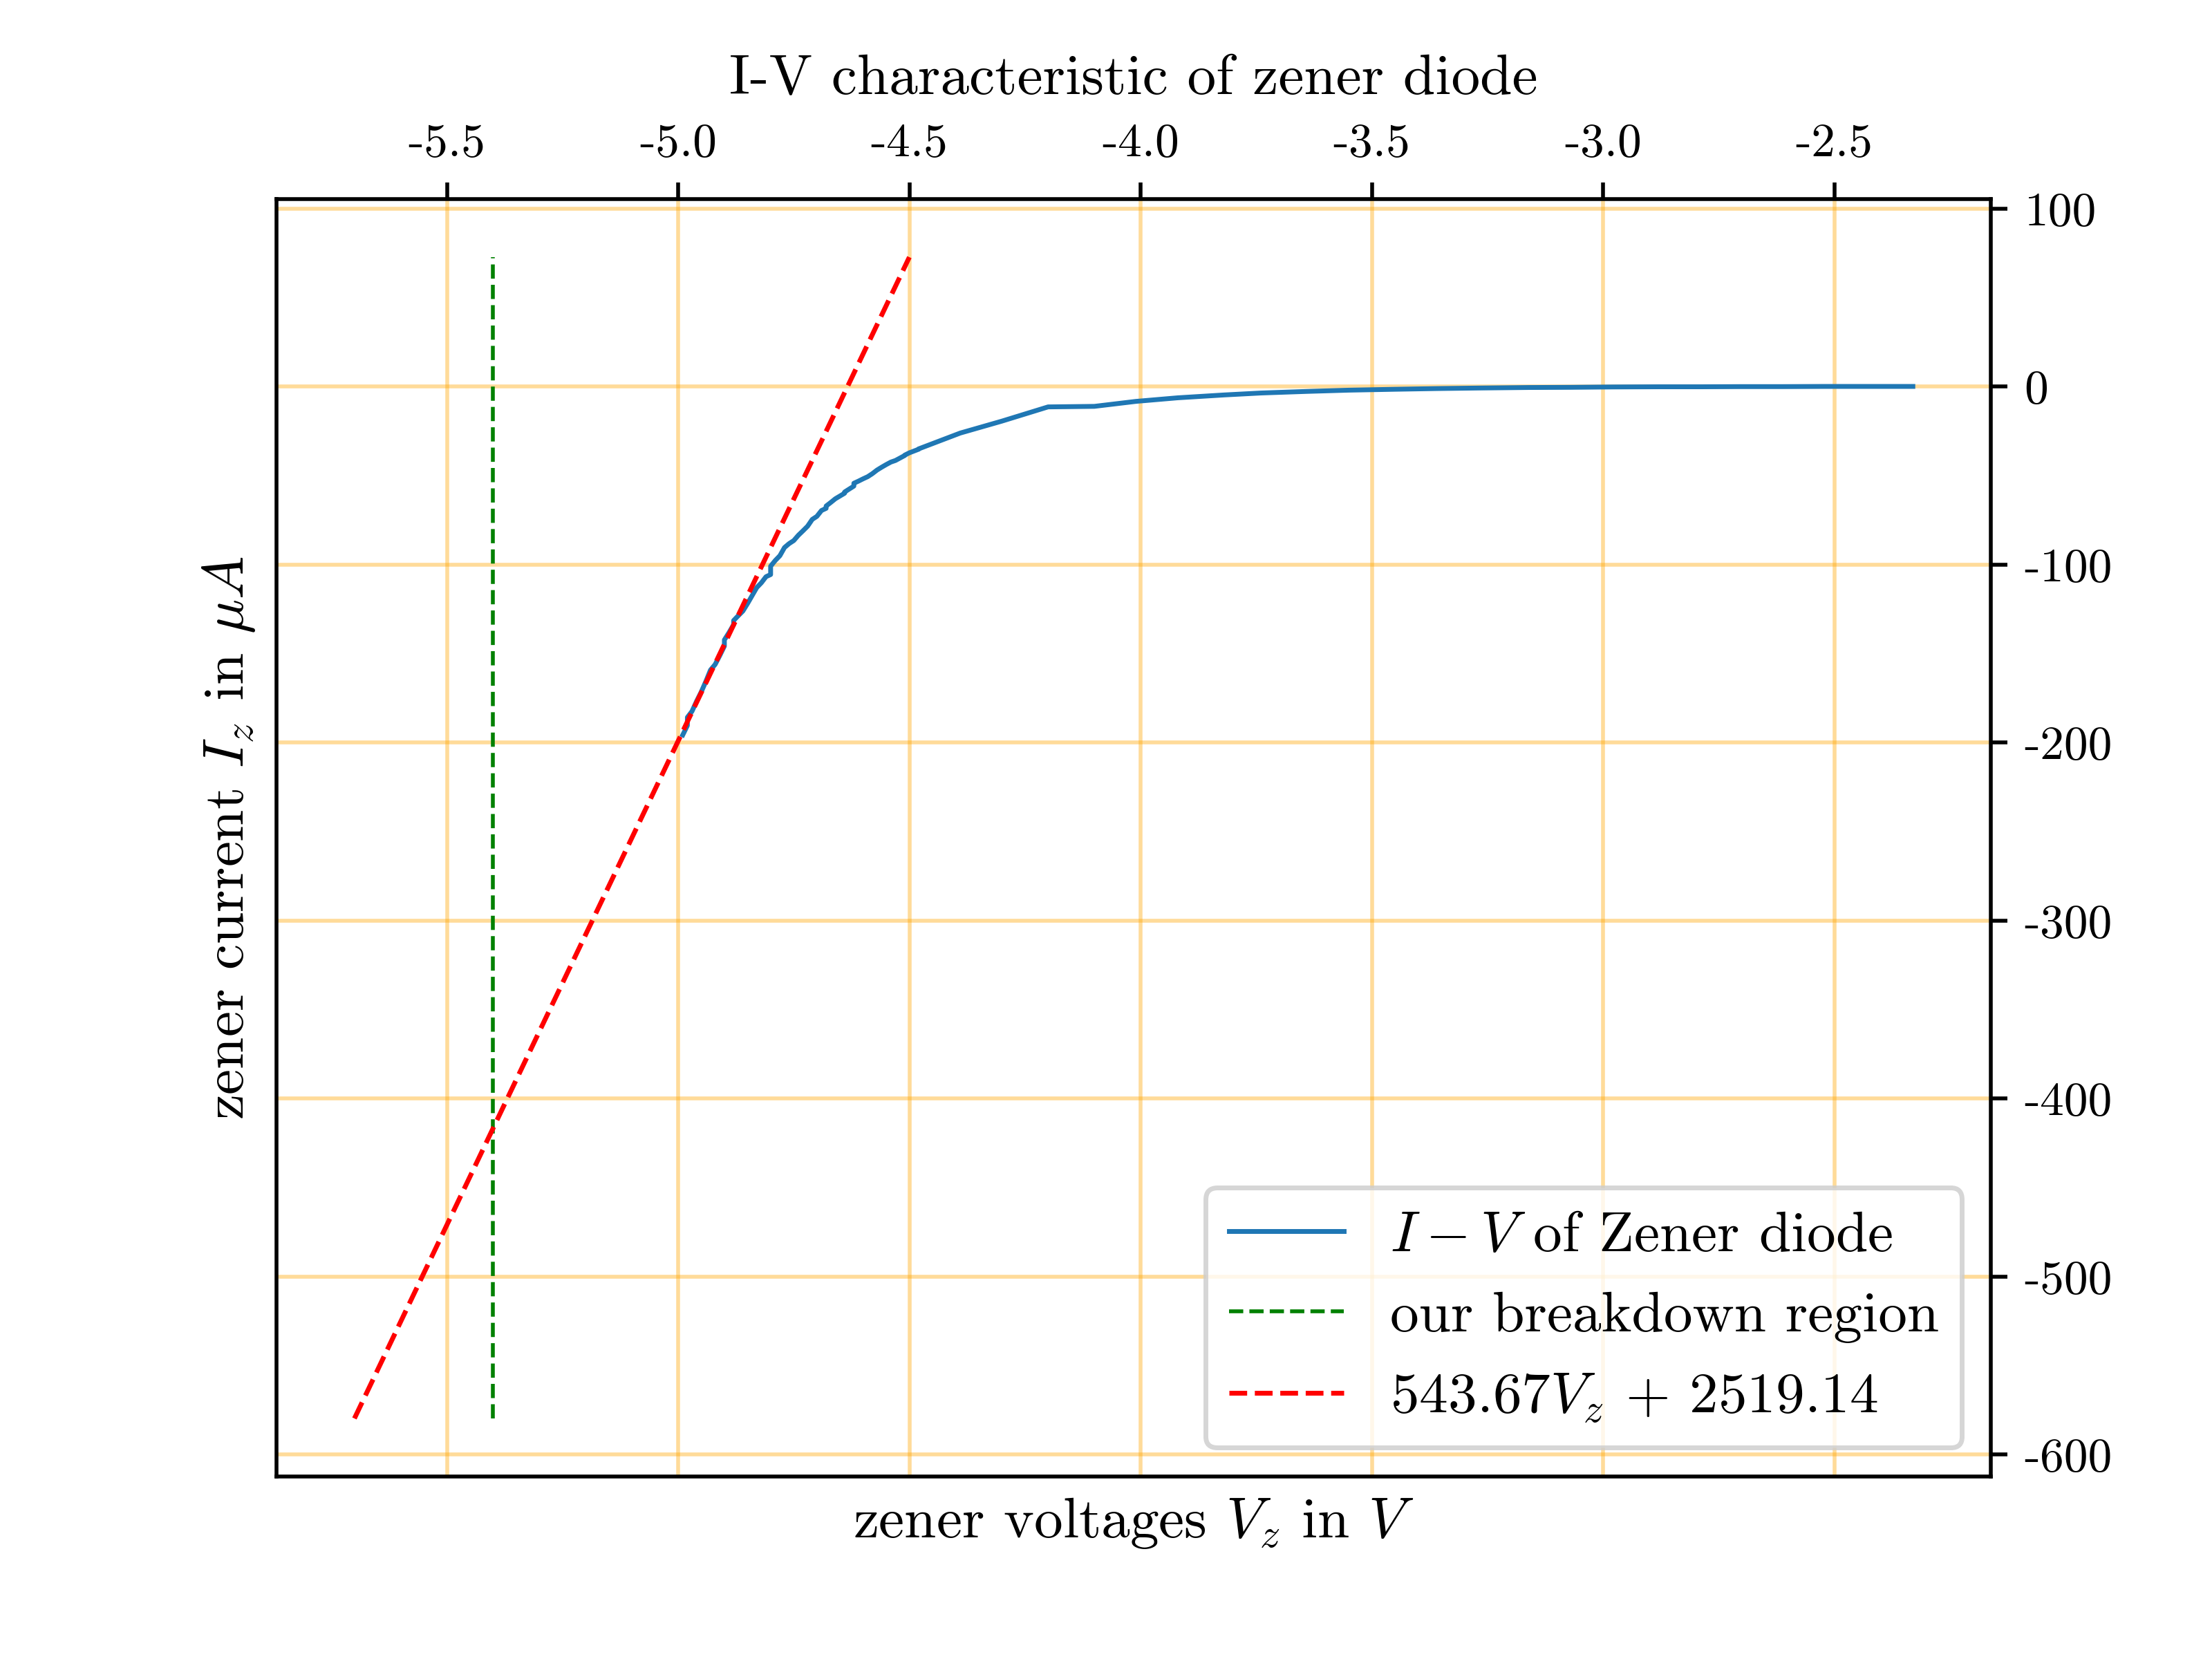
\includegraphics[width=1\textwidth]{zenerIV.png}}
\caption{current and voltage characterists of zener diode \label{exiv}}
\end{figure*}

Now, what we need is that fluctuation over the regulated DC voltage. These fluctuations have to be some function in the frequency domain as we assumed. This function must be made of different harmonics of sinusoidal waves with different phases and frequencies as thought by Fourier and his analysis. So basically we needed a system to measure different amplitudes of these harmonics at different frequencies to model our fluctuations. We needed a complete frequency spectrum at the particular bandwidth we are looking for in this analysis. The LOCK IN amplifier gives exactly that. 


\subsection{Measuring instrument: LOCK IN amplifier}

LOCK IN amplifiers came in the 1930s and became very important in signal extraction from given frequency and phase. It is very helpful in measuring signals in a very noisy environment. It takes two inputs, one which is being measured and one which is given as a reference mono frequency signal. Reference signal gets multiplied with input signal and gives output through a process called Phase sensitive detection in which it uses homodyne detection scheme and filters out signal as DC component. We will see in a bit.

\subsubsection{Phase sensitive detection}

In nutshell it uses frequency multiplication and generates double side bands which then pass through a low pass filter to extract signal. In figure \ref{psd} you can see a signal first goes into a low noise differential amplifier which strengthens the signal. Signal Gets multiplied by another reference signal. This gives rise to two bands which pass through a low pass filter which cancels higher degree signal and only left is low frequency signal.


\begin{figure}[hbt!]
\centering{\centering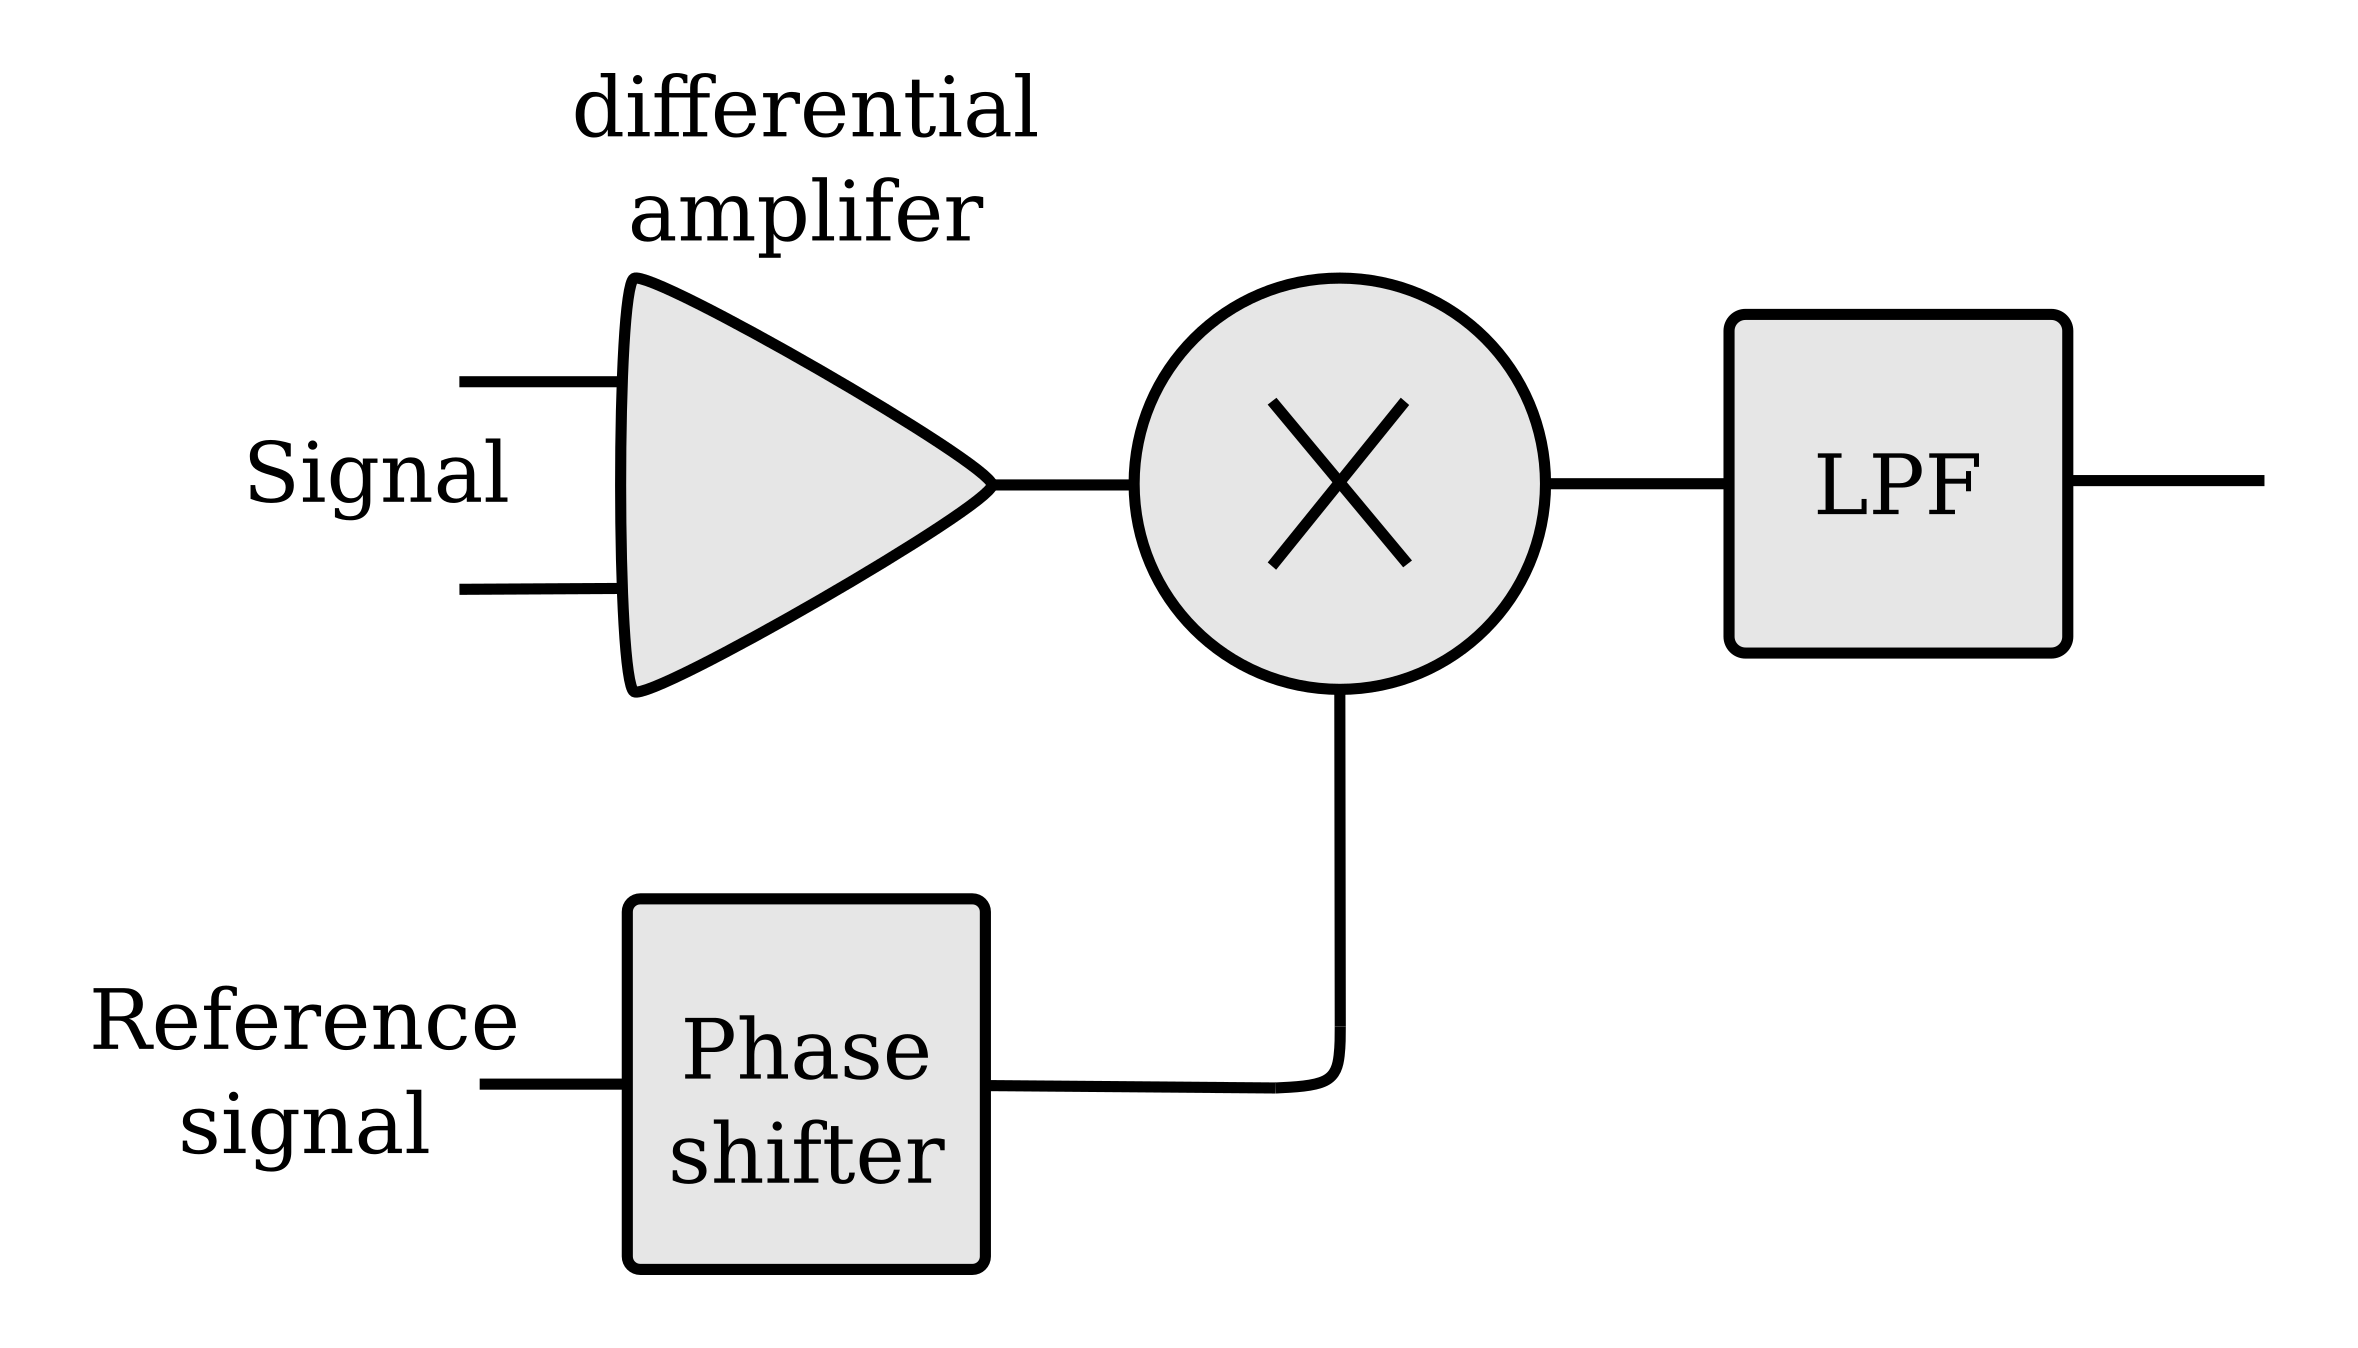
\includegraphics[width=.48\textwidth]{PSD.png}}
\caption{basic phase sensitive detector}
\end{figure}

If we take signal $V_s(t)$ with frequency $w_s$, amplitude $A$ and phase $\theta$. 

\begin{align*}
V_{s}(t) & = A \cos(w_st+\theta)\\
\\
& = \frac{A}{2} (e^{i(w_st+\theta)}+e^{-i(w_st+\theta)})\\
\end{align*}

Reference signal can be taken as following,

\begin{align*}
V_r(t) & = B (e^{-i(w_rt+\phi)})
\end{align*}

In common settings, $\phi = 0$ and $B=1$,

\begin{align*}
V_r(t) & = e^{i(-w_rt)}
\end{align*}

Together after mixing the signals we have,

\begin{align*}
Z(t) & = V_s(t)\timesV_r(t)\\
\\
& = \frac{A}{2}(e^{i\left[ (w_s-w_r)t+\theta \right]}+e^{-i\left[ (w_s+w_r)t+\theta \right]})\\
\\
& = X(t)+Y(t)
\end{align*}

Making $w_s=w_r$ which makes subtraction vanishes and only one term with higher frequency lefts. Passing this signal through a low pass filter with very low cutoff gives only DC components and rejects noise even from neighbouring frequencies.


\begin{align*}
Z(t) & = \frac{A}{2}(e^{i \theta})
\end{align*}

Two component $X(t)$ and $Y(t)$ becomes,

\begin{align*}
X(t) & =\re(Z(t))\\
\\
& =  \frac{A}{2}\cos(\theta)
\end{align*}

And,

\begin{align*}
Y(t) & = \im(Z(t))\\
\\
& =  \frac{A}{2}\sin(\theta)
\end{align*}

So, Amplitude and Phase becomes, 

\begin{align*}
R & = \sqrt{X(t)^2+Y(t)^2}\\
\\
& =  \sqrt{(\frac{A}{2}\cos(\theta))^2+(\frac{A}{2}\sin(\theta))^2}\\
\\
& = \frac{A}{2}\\
\\
\Theta & = \arctan(\frac{Y}{X})
\end{align*}

So, the final product in PSD is the absolute amplitude of the signal and its phase. 

\subsubsection{Time Constant }

\subsubsection{ENBW}

\subsubsection{Sensitivity} 

\subsubsection{LOCK IN amplifier over traditional measuring device/system}

For noise analysis LOCK IN amplifiers are the optimal choice. Traditional approaches deal with the first measurement of a small signal in the time domain. This signal gets amplified with additional noise from the amplifier. Also, amplifiers attenuates signals with its limited bandwidth which is a measure of concern for certain use case scenarios. This attenuated signal gets into some detector. For signal analysis, this signal must go into other  processes like analog to digital conversion then Fourier transformation. This whole process gives too much concerned noise which is not related to devices being analysed in our case the voltage regulator circuit. Alternative approach is to go with a LOCK IN amplifier. Which cancels out most burdens of traditional measurement steps. This whole combined help in reducing internal noise and increasing S/N ratio.
\\
\\
\emph{\large Pros of LOCK IN amplifier:}
\begin{itemize}
\item LOCK In amplifiers reduces attenuation of signal with increasing frequency since it does not measure signal in the whole frequency spectrum.
\item Increase S/N ratio over traditional amplifier circuit
\item Gives direct data into frequency domain
\end{itemize}\\
\\
\emph {\large Cons of LOCK IN amplifier:}
\begin{itemize}
\item Relatively expensive
\item Does not give information in time domain
\item Relatively slow for whole analysis of frequency domain (low but accurate resolution of frequency domain)
\end{itemize}

\subsection{SR830}

We used a LOCK IN amplifier from Stanford Research Systems. It is used to detect low amplitude signals as low as $10\frac{nV}{Hz}$ and frequency as low as $100mV$.  and measure very small AC signals - upto few nanovolts. Accurate measurements may be made even when the small signal is obscured by noise sources many thousands of times larger.


Internal block diagram of SR830,

%% \begin{figure*}[hbt!]
%% \centering{\centering\includegraphics[width=.55\textwidth,page=33,trim={5cm 5cm 5cm 10cm, clip}]{sr830m.pdf}}
%% \end{figure*}

\subsubsection{Inputs}

\subsubsection{Outputs}

\subsubsection{Interfacing}



Lock-in amplifiers use a technique known as
phase-sensitive detection to single out the component of the signal at a specific reference frequency and phase. Noise signals at frequencies other than the reference frequency are rejected and do not affect the measurements.


Now , on the basis of frequencies/ frequency levels and its origin, there are different types of noises are present in our environment. Some of them are discussed below:

